\documentclass[11pt, oneside]{scrartcl}   	% use "amsart" instead of "article" for AMSLaTeX format
\usepackage[top=2cm,right=2cm,bottom=2.5cm,left=2cm]{geometry}                		% See geometry.pdf to learn the layout options. There are lots.
\geometry{letterpaper}                   		% ... or a4paper or a5paper or ... 
%\geometry{landscape}                		% Activate for for rotated page geometry
%\usepackage[parfill]{parskip}    		% Activate to begin paragraphs with an empty line rather than an indent
\usepackage[parfill]{parskip}
\usepackage{graphicx}				% Use pdf, png, jpg, or eps§ with pdflatex; use eps in DVI mode
								% TeX will automatically convert eps --> pdf in pdflatex
\usepackage{amssymb}
\usepackage{amsmath}

\usepackage[TS1,T1]{fontenc}
%\usepackage{fourier, heuristica}
\usepackage{array, booktabs}
\usepackage[x11names]{xcolor}
\usepackage{colortbl}
\usepackage{caption}
\usepackage{bbm}
\usepackage{amssymb}
\usepackage{amsmath}
\DeclareCaptionFont{blue}{\color{LightSteelBlue3}}

\newcommand{\foo}{\color{LightSteelBlue3}\makebox[0pt]{\textbullet}\hskip-0.5pt\vrule width 1pt\hspace{\labelsep}}

\definecolor{light-gray}{gray}{0.7}

\title{Notes on Grobid}
\author{Joseph Boyd}
\date{}							% Activate to display a given date or no date

\begin{document}
\maketitle

Grobid (GeneRatiOn of BIbliographic Data) is a Java wrapper for applying conditional random fields (CRF) to the problem of metadata extraction of scientific papers. The wrapper sits atop a CRF engine that performs the abstract CRF computations. Wrapper and engine are combined through the use of the Java Native Interface (JNI). Grobid is divided into four packages: grobid-home, grobid-core, grobid-trainer, and grobid-server. Grobid produces a set of models, each addressing a different part of the metadata extraction, and each trained separately on its own spectrum of features. In the case of citation processing, the models are applied according to a hierarchy, starting with the segmentation of the reference list, followed by the tagging of each part of each reference, and finally a set of micro-models to further classify these reference parts.

\subsection{Engines}

Grobid allows for a choice between two alternative linear-chain CRF engines (both written in C++): CRF++ (developed by Taku Kudo) and Wapiti (developed by Thomas Lavergne). The default option is Wapiti, a more recent engine that allegedly performs better. Both engines follow similar input and output formats, allowing an easy abstraction within Grobid over the choice of engine. Though we have access to the source code, the CRF engine will be largely black-boxed in this project, and we will instead concentrate on tuning and configuring Grobid.

\subsection{grobid-home}

The grobid-home package houses the models, configuration files and additional software components such as pdftoxml, which is used to extract both plaintext and OCR data from the PDF inputs. This package does not contain any source code.

\subsection{grobid-core}

The grobid-core package contains the majority of the source code, including that for modelling documents and interacting with the CRF engine. grobid-core also supplies the main entry points for using Grobid as a command line tool. Through this interface, we may use Grobid to batch process collections of PDF files.

\subsection{grobid-trainer}

grobid-trainer contains the source code for coordinating the training of the models, including preparing the training data from the TEI inputs. grobid-trainer provides the main entry point for training models and can also be used for training models through the command line.

\subsection{grobid-server}

grobid-server onsists of a web interface for Grobid, running on Jetty (Java) HTTP server. It allows a user to upload a PDF through a web form for processing. This feature is unlikely to be of any interest to this project.

\subsection{Models}

\begin{figure}[!ht]
\center
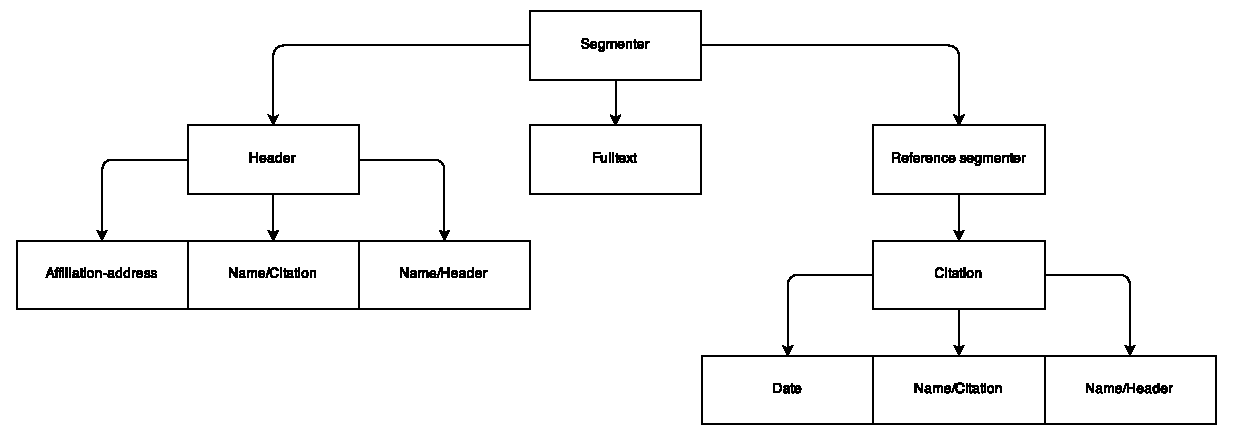
\includegraphics[width=7in]{figures/cascade.pdf}
\caption{Cascade of models used by Grobid}
\label{fig:cascade}
\end{figure}

Finding the header is typically easy, as we can assume it always to constitute the first page or so of the document. For this reason, when we call \texttt{processHeader} on its own, the Segmentation model is not called. On the other hand, though references are almost invariably at the end of an article, it is difficult to guess where it begins, and the reference model would suffer more from garbage than the header model. For this reason, the Segmentation model is called when we call \texttt{processReferences}, before calling the Reference-segmenter model to slice the reference list (identified by Segmentation) into individual citations.

Grobid manages the training, evaluation and usage of a set of models, each addressing a part of the information extraction. Higher level models such as the Header, Segmentation, and Reference Segmentation models may applied directly to PDFs, while the other, more specific models, such as the Date model, operate only on plaintext inputs. Though they have much in common, the models vary in the labels they assign, the features they exploit, and, due to the varying size of the vocabulary (compare say, the number of possible month names to the number of possible author names), the size (dimensionality) of the models. Calling \texttt{processFullText} runs all available models on a batch of PDF documents. The output of training is a model, which takes takes the form of a text or binary file, depending on the engine. These models are then ``loaded'' at prediction time for the labelling of new documents. Some models are in practice not used independently, rather, they form part of a ``cascade'' of models that progressively address finer subcomponents of the classification problem. As shown in Figure \ref{fig:cascade}, reference extraction begins with segmentation models, which classify each line of a document, resulting in homogenous blocks of lines e.g. header, paragraph, figure, references. This information is then distributed to the other models, for example the Reference Segmentation model, which further breaks down the reference list into individual references. The Citation model then classifies the parts of each reference into classes, for example, date, affiliation, and author. Finally, the atomic subcomponents of these are classified by their respective models. Note that the citation branch of the hierarchy has the option of further cross-checking extracted references with the third-party CrossRef web service.

\subsection{Training}

Both training and evaluation are performed on sets of XML documents following the Text Encoding Initiative (TEI) standard for representing electronic texts (http://www.tei-c.org/index.xml). This is also the output format for prediction, so there is consistency between input and output formats. It may appear paradoxical to \emph{evaluate} on well-structured data, when the tool is ultimately intended to operate on unstructured PDF documents, that is, at prediction time. However, with closer inspection of the source code, an equivalence can be seen between:

\begin{enumerate}
\item applying an OCR tool (pdftoxml), tokenising the output and transforming to CRF input data
\item extracting tokens from TEI documents, and transforming to CRF input data
\end{enumerate}

\begin{figure}
\begin{verbatim}

[...]

January january J Ja Jan Janu y ry ary uary LINESTART INITCAP NODIGIT 0 0 1 NOPUNCT I-<month>
1994 1994 1 19 199 1994 4 94 994 1994 LINEEND NOCAPS ALLDIGIT 0 1 0 NOPUNCT I-<year>
 
July july J Ju Jul July y ly uly July LINESTART INITCAP NODIGIT 0 0 1 NOPUNCT I-<month>
1996 1996 1 19 199 1996 6 96 996 1996 LINEEND NOCAPS ALLDIGIT 0 1 0 NOPUNCT I-<year>

[...]

\end{verbatim}
\caption{Training input for Wapiti}
\label{fig:traininput}
\end{figure}

\begin{figure}
\begin{verbatim}
# Capitalization
U50:%x[0,11]
U51:%x[1,11]
U52:%x[-1,11]
U53:%x[0,11]/%x[1,11]
U54:%x[-1,11]/%x[0,11]
\end{verbatim}

\caption{Feature templates for Wapiti}
\label{fig:template}
\end{figure}

Both approaches yield the same input data for the CRF engine, and so evaluation is in fact equivalent to prediction, despite the initial difference in input formats. Figure \ref{fig:traininput} shows an excerpt from an input file to the CRF engine for training. These features are for inputs ``January 1994'' and ``July 1996'', for training the Date model. The features range from token identity, to a variety of prefixes and punctuation features. It should be noted that OCR information is only used in higher level models, that is, the Header and Segmentation models. The input for lower-level models such as Date is plaintext, and so features are typically simple, but dictionary-based features, where information about a token is referenced in a dictionary resource within Grobid, are also used. Note the features shown are only those pertaining to the token itself. The full range of features (including those involving concatenations of the token's neighbours etc.) are defined by a set of feature templates. The feature templates for each model are contained in a separate file. An excerpt of this is shown in Figure \ref{fig:template}. These are given as a separate input to the CRF engine, and it is with these that the engine constructs all feature functions for the model. It is therefore vital that the feature extraction, which is generated by Grobid, is aligned with the template file, which is manually configured by the developer. As depicted in Figure \ref{fig:flow}, there is a strong coupling between these two parts of Grobid. The excerpt shown is from the Wapiti model, but the notation is the same for CRF++, which first standardised the syntax. This subset of five feature templates capture information about the capitalisation of a token and its neighbours. The notation has the structure, [identifier]:[\%x][row, col], where row is the offset from the current token, and col indicates the feature index. Thus, ``U50:\%[0,11]'', denotes that the feature template identified as ``U50'' takes the 11th feature for the current token (0 offset). This feature will be equal to 1 if a token is capitalised, and 0 otherwise. ``U52:\%[-1,11]'' indicates the same thing, but based on the capitalisation of the \emph{previous} token. ``U54:\%x[-1,11]/\%x[0,11]'' is a binary function for detecting the capitalisation of the current \emph{and} the following token.

Now we may see an alignment with the mathematical model. Recall a linear chain CRF is expressed in the simplest case as,

\begin{equation}
p(\textbf{y}|\textbf{x}) = \frac{p(\textbf{x}, \textbf{y})}{\sum_{y'}{p(\textbf{x}, \textbf{y}')}},
\end{equation}

where, 

\begin{equation}
p(\textbf{x}, \textbf{y}) = \text{exp} \Bigg\{\sum_t{
\sum_{i, j \in S}{
\lambda_{ij}\mathbbm{1}_{\{y_t = i\}}\mathbbm{1}_{\{y_{t-1} = j\}}
}
+ \sum_t\sum_{i \in S}\sum_{o \in O}{
\mu_{io}\mathbbm{1}_{\{y_t = i\}}\mathbbm{1}_{\{x_t = o\}}
}
}\Bigg\},
\label{eq:joint}
\end{equation}

Here $\textbf{x}$ is a sequence of observations and $\textbf{y}$ is a sequence of labels. $S$ is the set of all labels, $O$ is set of observations (the vocabulary of the tokens to be labelled). When the coefficients $\lambda_{ij} = \log p(y_t=i, y_{t - 1}=j)$ and $\mu_{ij} = \log p(y_t=i,x_t=o)$, this joint distribution is equivalent to a Hidden Markov Model (HMM), with coefficients, $\lambda_{ij}$ as transition probabilities and $\mu_{ij}$ emission probabilities. In this simple case, features are based solely on the token's identity, i.e. feature functions are an indicator function. For clarity, we may write,

\begin{equation}
p(\textbf{x}, \textbf{y}) = \text{exp} \Bigg\{
\sum_{i \in S}
\sum_{j \in S}
\lambda_{ij}
%\sum_t
%\mathbbm{1}_{\{y_t = i\}}\mathbbm{1}_{\{y_{t-1} = j\}}
F_{ij}(\textbf{y})
+ 
\sum_{i \in S}
\sum_{o \in O}
\mu_{io}
%\sum_t
%\mathbbm{1}_{\{y_t = i\}}\mathbbm{1}_{\{x_t = o\}}
F_{io}(\textbf{x}, \textbf{y})
\Bigg\},
\label{eq:joint}
\end{equation}

where $F_{ij} = \sum_t\mathbbm{1}_{\{y_t = i\}}\mathbbm{1}_{\{y_{t-1} = j\}}$ and $F_{io} = \sum_t\mathbbm{1}_{\{y_t = i\}}\mathbbm{1}_{\{x_t = o\}}$. In a CRF, however, we may replace the indicator function for observations with any sort of function, typically binary, extracting rich features from a token. Thus, $F_{io} = \sum_t\mathbbm{1}_{\{y_t = i\}}f_{io}(\textbf{x})$. The set of functions, $\{f_{io}\}$, are the functions that we define in the feature template files. Note that, unlike an HMM, the vocabulary is not pre-defined, it is ``discovered'' through training on samples. Therefore, the number of actual features depends on the training set itself, whereas the feature template is fixed. Since we use indicator functions, which produce a feature for every observation, we may end up with an enormous number of features. Take the Date model for example: 5815 features are produced for a single block (not counting the one representing the label), and there are seven labels. As per our formulation in (\ref{eq:joint}) we therefore have 7 * 7 ``transition'' features and 5815 * 7 ``emission'' features, totalling 40754 features. This is corroborated by the model output in Figure \ref{fig:output}. Wapiti automatically constructs this vast feature space from the inputs we provide. In the Date model, the labels are I-<day>, I-<month>, I-<year>, I-<other>, <day>, <month>, and <other>. The I (probably) stands for ``initial'', as in training these are assigned to the first tokens of this class found in the string.

\begin{figure}
\begin{verbatim}
* Initialize the model
* Summary
    nb train:    493
    nb labels:   7
    nb blocks:   5816
    nb features: 40754
* Train the model with l-bfgs
  [   1] obj=1688,58    act=16482    err=25,80%/50,91% time=0,08s/0,08s
  [   2] obj=1221,30    act=15580    err=19,11%/35,50% time=0,05s/0,12s
  [   3] obj=922,15     act=13869    err=17,20%/33,67% time=0,04s/0,17s
  [   4] obj=638,04     act=10845    err= 6,53%/15,21% time=0,04s/0,20s
  [   5] obj=478,72     act=10582    err= 5,68%/13,59% time=0,04s/0,24s
  [   6] obj=416,15     act=9926     err= 3,77%/ 9,53% time=0,04s/0,28s
\end{verbatim}
\caption{Output from training date model}
\label{fig:output}
\end{figure}

A model is typically a large file (as much as 100Mb). At the top of the file, the feature templates are declared, just as they are in the input. Because of this, that file is not required at prediction time. Following this the labels are declared. Then come two longer sections: first, the feature functions themselves as defined. Figure \ref{fig:model} shows the first 12 features produced from the first token in the first sample in the training set--``November''. Because this is the first token in the string, we see the first three feature macros, which relate to the identity of the token's predecessors, remain unresolved. The fourth, however, shows the indicator for the token. This function will be true if a token is equal to ``November''. The fifth function is an indicator for if the token's successor is equal to ``19'', and so on. The final (and usually largest) section of the model file defines the non-zero weights for the feature functions. The weights are represented in scientific notation and in hexadecimal representation, presumably to avoid arithmetic underflow (a common problem when dealing with with the computation of HMMs and related models).

\begin{figure}
\begin{verbatim}
8:u00:_x-3,
8:u01:_x-2,
8:u02:_x-1,
12:u03:November,
6:u04:19,
5:u05:,,
8:u06:2001,
17:u07:_x-1/November,
15:u08:November/19,
8:u09:19/,,
13:u0A:_x-2/_x-1,
8:u10:_x-2,
8:u11:_x-1,
\end{verbatim}
\caption{Excerpt of model contents--the realisation of feature functions}
\label{fig:model}
\end{figure}

\subsection{Evaluation}

Training may be done with a split defined by the developer, which Grobid will use to set aside a proportion of the training data for evaluation. The evaluation of a model produced by training follows identical procedures, preparing the same input data. The output, however, is not a model but a the input data with labels. Grobid compares its predictions with the ground truth and outputs \emph{precision}, \emph{accuracy} and \emph{F1 scores} as performance indicators, at the token, field, and instance levels. A token refers to a single contiguous string of characters (without spaces), a field is a block of contiguous tokens, and an instance is an entire document. Accuracy of an instance is therefore judged by the correctness of all tagging for the whole document, a difficult thing to achieve without any mistakes.

\subsection{Prediction}

Figure \ref{fig:flow} shows the flow of information from input to output, as well as the relationship between training and prediction. When it comes to labelling (prediction), the starting point is a PDF document. With a third-party tool, pdftoxml, this is transformed into an XML file containing OCR information (font, style, orientation) for every token in the document. This information is stored in LayoutToken objects within Grobid. These tokens are arranged into blocks and features are extracted as they were for training and evaluation. Excepting the absence of tokens, the input is the same. The model created in the training phase is first loaded, and then the EngineTagger calls the CRF engine to label the inputs. Unlike for training, the feature template file is not required, as these have already been absorbed into the model file. After processing, Wapiti returns the same file with tags inserted. Grobid then further processes this information to transform it into the final TEI format.

\begin{figure}[!ht]
\center
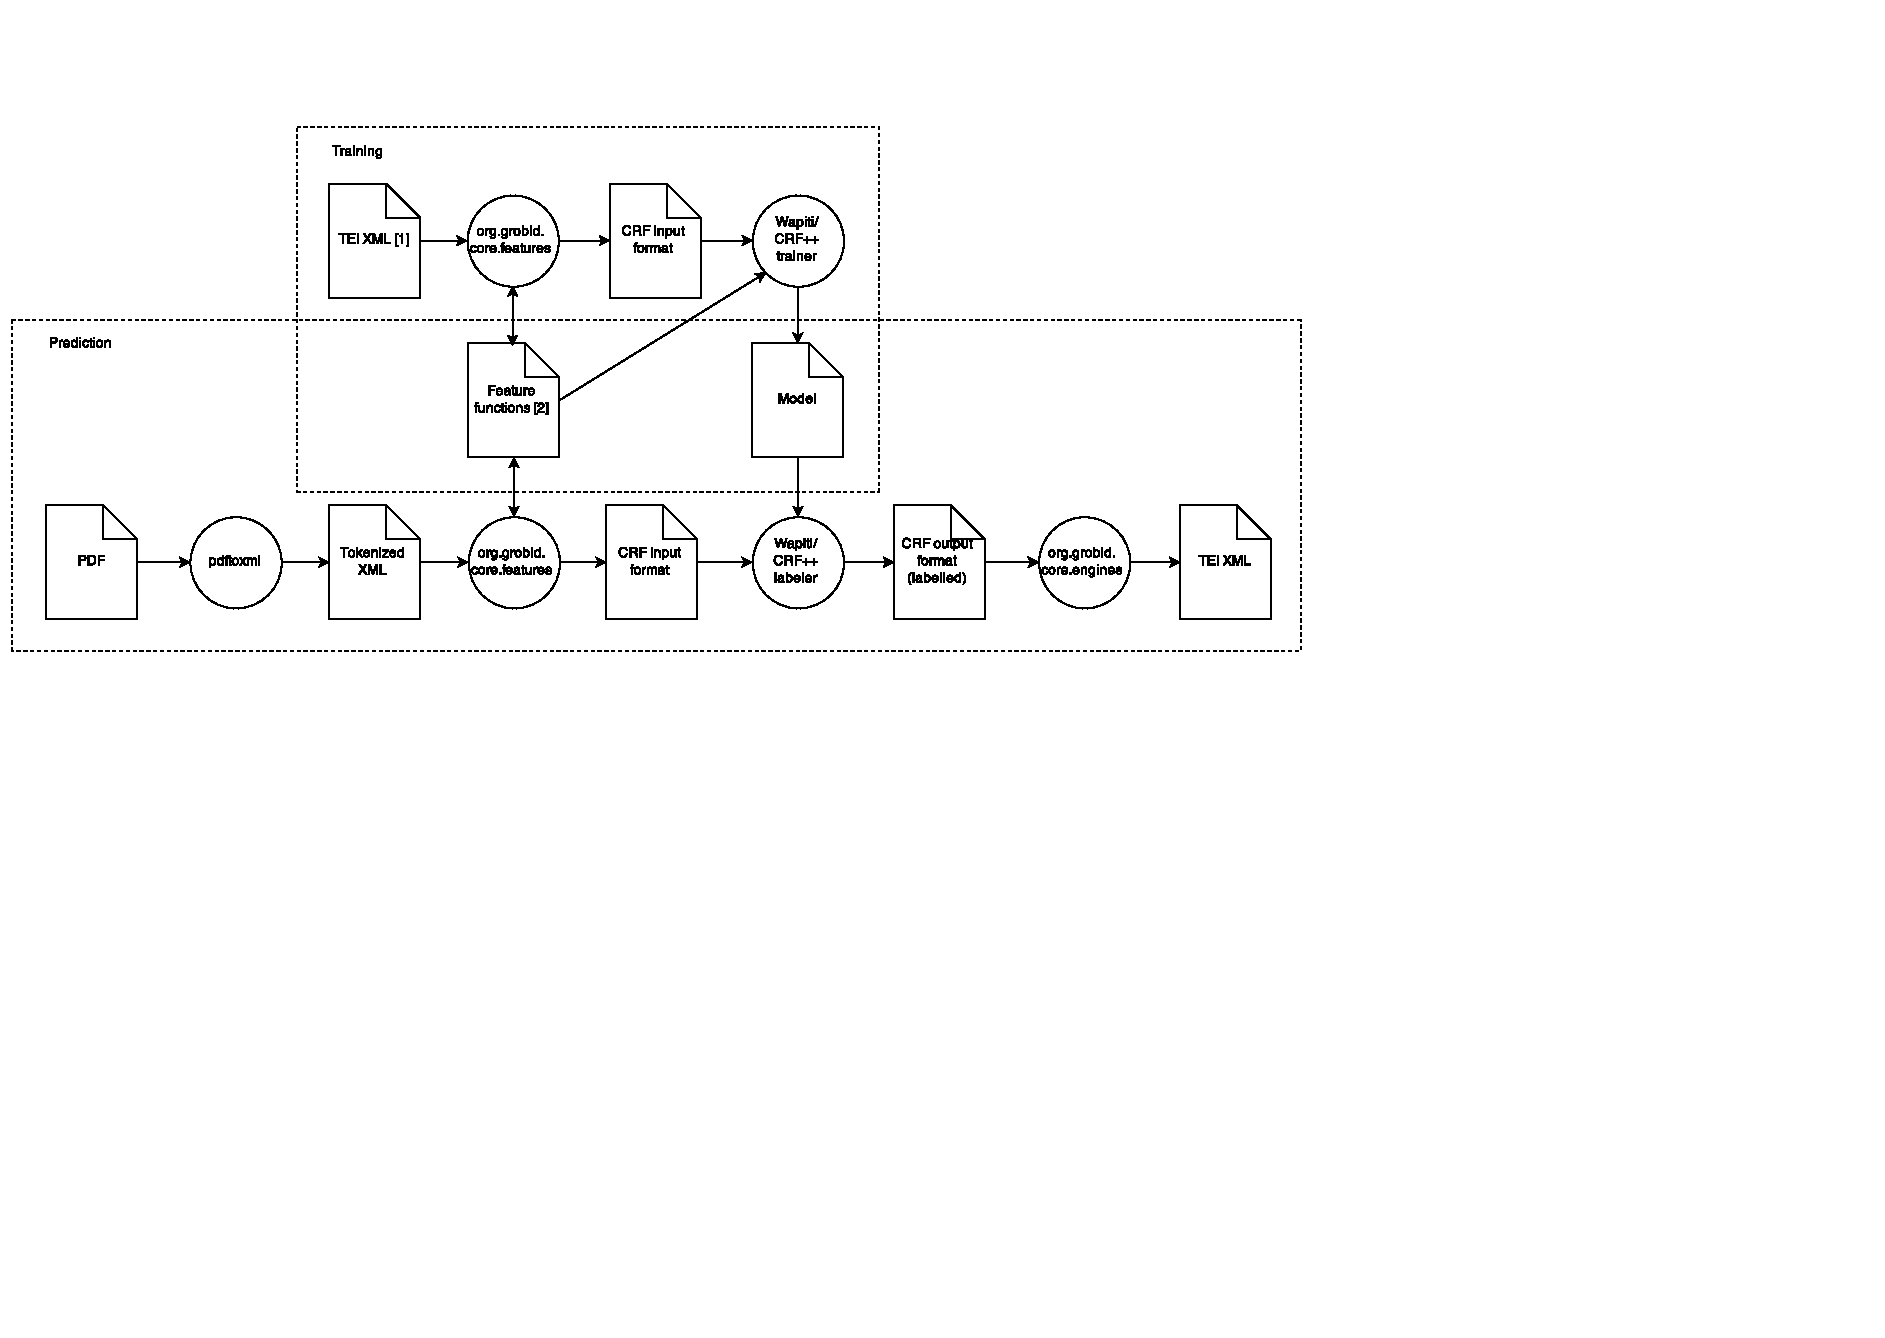
\includegraphics[width=7in]{figures/grobid.pdf}
\caption{The flow of information and the interaction of training and prediction. [1] Training inputs follow and TEI standard. [2] There is a strong coupling between the features module and the feature functions file.}
\label{fig:flow}
\end{figure}

\subsection{Other Functionality}

In addition to the above, Grobid provides a means of producing training sets semi-automatically. This consists of applying the existing models on the training set to produce the XML inputs. Of course, each field must be checked against a ground truth and errors corrected before it is used as a training set. We intend to use this functionality to generate training data for benchmarking Grobid on HEP papers.

These methods are,

\begin{enumerate}
\item createTrainingHeader
\item createTrainingFulltext
\item createTrainingSegmentation
\item createTrainingReferenceSegmentation
\item createTrainingCitationPatent
\end{enumerate}

Now, for example, when we run \texttt{createTrainingHeader} to create a header training set, grobid creates four files per pdf:

\begin{enumerate}
\item PDF-NAME.affiliation.tei.xml
\item PDF-NAME.authors.tei.xml
\item PDF-NAME.header.tei.xml
\item PDF-NAME.header
\end{enumerate}

Files (1) and (2), are the training data for the affiliation-address and author models respectively. Files (3) and (4) are jointly required for training the Header model: file (3) simply contains the tagged data, but file (4) contains the feature (untagged) for each token, including OCR information. We must additionally store (4) as the OCR information cannot be derived from the plaintext TEI file. That the processing does not tag the blocks allows the programmer to intervens and correct and discrepancies with the ground truth. Thus the header files need only be corrected then moved to a separate folder for training. Notice training data for the segmentation models may be harder to generate automatically.

Notice that there is no method for creating citation training data, $\mathcal{D}_{tr}$ directly. This data is created as part of \texttt{createTrainingFulltext}. This creates four files also:

\begin{enumerate}
\item PDF-NAME.training.citations.authors.tei.xml
\item PDF-NAME.training.references.tei.xml
\item PDF-NAME.training.fulltext.tei.xml
\item PDF-NAME.training.fulltext
\end{enumerate}

File (1) contains a refinement of the author names found in file (2), thus can be used as training data for the Name-citation model. File (2) contains the training data for the Citation model, in the format apparent in the training corpus. As should be expected, the name and date fields for this data are not resolved into their subcomponents, this task being left to the smaller models dedicated to these tasks. Files (3) and (4) are the files required for training the citation model.

\begin{center}
\begin{table}
\begin{tabular}{ | p{0.2\linewidth} | p{0.8\linewidth} |}
	\hline
	Model & Labels \\ \hline
    	Header & <title>, <author>, <affiliation>, <reference>, <submission>, <abstract>, <address>, <keyword>, <degree>, <pubnum>, <email>, <date>, <copyright>, <intro>, <web>, <note>, <phone>, <dedication>, <entitle>, <grant>, <date-submission> \\ \hline
	Affiliation address & <institution>, <other>, <settlement>, <department>, <postcode>, <contry>, <marker>, <region>, <addrLine>, <laboratory>, <postbox>, <other>, <null> \\ \hline
	Name/Header & <forname>, <surname>, <marker>, <middlename>, <other>, <suffix>, <title> \\ \hline
	Name/Citation & <surname>, <forname>, <other>, <middlename> \\ \hline
	Citation & <journal>, <volume>, <other>, <issue>, <pages>, <date>, <author>, <title>, <booktitle>, <location>, <pubnum>, <note>, <publisher>, <editor>, <institution>, <tech>, <web>, <issue> \\ \hline
	Date & <other>, <day>, <month>, <year> \\ \hline
	Segmentation & <headnote>, <header>, <body>, <page>, <references>, <footnote>, <cover>, <acknowledgement>, <annex> \\ \hline
	Reference-Segmenter & <label>, <reference>, <other> \\ \hline
	Fulltext & <section>, <paragraph>, <citation\_marker>, <other>, <table\_marker>, <figure\_marker>, <figure\_head>, <trash>, <figDesc>, <equation>, <item> \\ \hline
\end{tabular}
\caption{We have here excluded the Patent, Entities, and E-book models as these are experimental models not currently used by Grobid. Of the models listed, we will be focusing on Header, probably Segmentation, and perhaps Reference-Segmenter and Citation also. This is because these are likely to require special training and configuration for HEP papers. Others such as Name and Date are unlikely to improve with training on HEP papers.}
\label{fig:featurelist}
\end{table}
\end{center}

\begin{figure}
\begin{verbatim}
<?xml version="1.0" encoding="UTF-8"?>
<tei xmlns="http://www.tei-c.org/ns/1.0" xmlns:xlink="http://www.w3.org/1999/xlink"
 xmlns:mml="http://www.w3.org/1998/Math/MathML">
<teiHeader><fileDesc><sourceDesc><biblStruct><analytic>
	<author>
		<persName>
			<forename>B</forename>.
			<surname>GARRIGUES</surname>
		</persName>
		ET
		<persName>
			<forename>A</forename>.
			<surname>MUNOZ</surname>
		</persName>
	</author>
</analytic></biblStruct></sourceDesc></fileDesc></teiHeader>
</tei>
\end{verbatim}
\caption{Sample TEI (input and output) format for the Name-header model.}
\label{fig:traininput}
\end{figure}

%
%For each model, there is a template of "macros" (grobid-trainer/resources/dataset/[MODEL]/crfpp-tempates/) which follow a format common to Wapiti and CRF++. These macros describe feature "templates" which may be expanded into the many features functions of the model...
%
%
% these deriving primarily from the "token" features--those features based on presence of a particular string. The number of actual features therefore depends on the training set itself, whereas the feature template is fixed (these correspond to the feature functions in the literature).
%
%The feature template file is therefore passed to the CRF engine, along with a file that is derived from the training corpus (placed in grobid-home/tmp). The feature template file must be provided, and constitutes part of the feature engineering effort. There must be some part of the code reflecting this................... yes, it is the, for example, FeaturesVectorDate. However, the .train and .test files only extract the features corresponding with the [0, X] template, i.e. the current row (0 offset), and . Features corresponding to a non-zero offset (i.e. those constituting a link between different tokens) are only expressed implicitly through the feature template i.e. are not enumerated in the .train/.test files (this is left up to the CRF engine). What about label features????? These are included too, and they correspond to the "output" template (presumably) and is also added by the FeaturesVector module.
%
%The model is a much larger text file which begins with listing the feature templates found in the feature template file, followed by a list of labels. The structure is a little more mysterious, but we see each of the features of the training examples are presented sequentially (strictly speaking, this shouldn't correspond directly to the training samples, for example if two samples where the same, they should not both be represented......... [TODO: return to the CRF tutorials]). Anyhow, we see a comment (or special label) indicating the next 6597 lines represent features... These are what are referred to as "blocks" by the training output. Labels = 7, though it is not yet clear why I-<month> is different from <month>. nb train (619) refers to the number of samples. Note that, though we have only 341 tei files, some contain more than one date sample. Now, from lines 61 to 222 (?) we have features corresponding to the first sample..... It seems as though when we have for example:
%
%8:u00:\_x-3,
%8:u01:\_x-2,
%8:u02:\_x-1,
%
%This indicates the macro (feature template) is unresolved, as clearly in the case of the first token, there is no previous, nor two before, nor three before token. N.B. this does not imply a higher-order Markov condition... these offsets are over the input variables, moreover this doesn't imply a more complex dynamic programming (Viterbi) prediction method. The puzzling thing is then, why are these not present for the following case (10 April 2008)? Features such as INIT/NOCAPS must represent INIT "GIVEN" NOCAPS... Note, this is not then repeated in the model--once a feature has been represented, it is not repeated. We do however have 12 other features corresponding to this feature template, for example, NOCAPS/ALLCAP, and NOCAPS/INITCAP, and every other combination discovered in the training data (though not all possible combinations--these are implicitly modelled as having zero probability). These are, incidentally, exhausted rather early in the model file, as it shouldn't take long to see all of the (most likely) combinations in the first few data samples. The label is represented as a feature only once:
%
%1:b,
%
%i.e. right at the beginning. Thus, the first 57 feature are those features centered on the first token--"May". Following this is the second token, but now we have
%
%8:u00:\_x-2,
%
%i.e. x-3 for the second token, which is x-2 of the first. Then there is x-1 for x-2, and an actual token "May", for x-1 (the previous token).
%
%And so it continues for the current data sample. But now, when we arrive at the next sample, we find we have already covered the first three features in the previous example:
%
%i.e. here u00 would give x-3 again etc., and so the first feature listed derived from this data sample is,
%
%6:u03:10,
%
%on line 231, corresponding to "10 April 2008"
%
%and so it continues, and we have it that features from the second sample occupy lines 231-283 (53 lines), 284-336 (53 lines) etc. and one of the last samples "October 2003" has only two features! Of course it's likely some samples (duplicates) yielded no features at all. This therefore gives the intuition that increasing the training set for something such as date would experience diminishing returns very quickly.
%
%The first line in the model is a comment:
%
%\#mdl\#2\#10960
%
%indicating "model", 2 (???--perhaps indicating binary inputs), 10960 weights 
%
%* * *

\subsection{Pipeline}

\subsection{Training - References}

To prepare Grobid for practical reference extraction, our task is twofold, involving the training of both the \texttt{reference-segmenter } and \texttt{citation} models. The overall success of the citation model in tagging an entire reference list depends on the reliability of the citation blocks fed to it by its parent model. To illustrate, even a citation model that is perfect in its own right will not help very muchin the reference extraction if the \texttt{reference-segmenter} above it is incapable of finding the references. Note that, to be precise, there is a further dependency on the accuracy of the \texttt{segmenter} model, the most high-level model in Grobid's arsenal, which is responsible for identifying the reference section for the before it is segmented, however we will assume temporarily that this is accurate enough in practice. \emph{Instance-level} accuracy for the citation model, measured over a whole document, will be the number of correctly tagged references \emph{as a fraction of} the references correctly found by the \texttt{reference-segmenter}.

\begin{figure}
\begin{verbatim}
<bibl>
<label>[20]</label>
D. A. Hill, " Fields of horizontal currents located above the earth, " IEEE Transactions
on Geoscience and Remote Sensing, vol. 26, no. 6, pp. 726-732, 1988. [21] 
A. M. Badescu, V. Savu, and O. Fratu, " Preliminary tests in Unirea salt mine (Slanic
Prahova, Romania), " Report 4, University Politehnica of Bucharest, Bucharest,
Romania, 2011.
</bibl>
<bibl>
<label>[22]</label>
M. Stefanescu, O. Dicea, and G. Tari, " Influence of extension and compression on
\end{verbatim}
\caption{Sample error made by the (cora-trained) \texttt{reference-segmenter} model: the model fails to spot the citation label for reference [21], and the references are consequently merged. The \texttt{citation} model will then fail to match the ground truth.}
\label{fig:segerror}
\end{figure}

By contrast, the training of these two models may be performed independently. It does not matter to the citation model if the references in its training set are not contiguous members of the same reference list; the \texttt{citation} model operates at the reference string level. For this reason, creating our training set (as per the pipeline) for the citation model is simplified: if, when preparing the set, we notice a ground truth reference is missing from the output, we can just ignore this and continue. On the other hand, it matters very much that the \texttt{reference-segmenter} identifies the correct number of references, as this is the goal of the model, and it has a knock-on effect for the \texttt{citation} model below it. See for example Figure \ref{fig:segerror}, showing an error made by the pre-trained (Cora) \texttt{reference-segmenter} model shipped with Grobid.  It is rather surprising that such obviously strong indicators as the square brackets in the citation label, ``[21]'', are insufficient to classify it as such, especially when this error seems to happen rather often. This may be the result of poor feature engineering, a limited test set, or a mixture of the two.





\end{document}



